\section{Experiments}
We evaluate the proposed stopping-calibration procedure in two complementary settings. 
In \cref{sec:experiments_1}, we consider fixed acquisition trajectories across vision and medical-imaging benchmarks to assess whether the method controls the target risk while reducing the number of measurements acquired. 
In Section \ref{sec:experiments_2}, we extend the evaluation to learned adaptive acquisition policies by applying our method as a post-hoc wrapper around JAFA (Shim et al., 2018), a reinforcement-learning-based acquisition model. 
We assess whether the wrapped system controls the target risk while retaining the efficiency of the underlying adaptive policy.
%We evaluate \gls{method} in two complementary settings. In section-\ref{sec:experiments_1}, we study its behavior on a diverse set of sequential acquisition problems under fixed acquisition trajectories. The goal of this section is to assess whether the proposed method achieves the desired risk control while retaining practical stopping efficiency across vision and medical-imaging benchmarks. In section \ref{sec:experiments_2}, we demonstrate that our method is complementary to learned adaptive acquisition policies by wrapping them around a reinforcement-learning-based acquisition backbone, JAFA \citep{jafa-2018}, and evaluating whether the resulting wrapped system preserves the desired risk guarantees while retaining the efficiency of the underlying adaptive policy.

\begin{figure}[h]
    \centering
    \begin{minipage}[t]{0.4\linewidth}
        \centering
        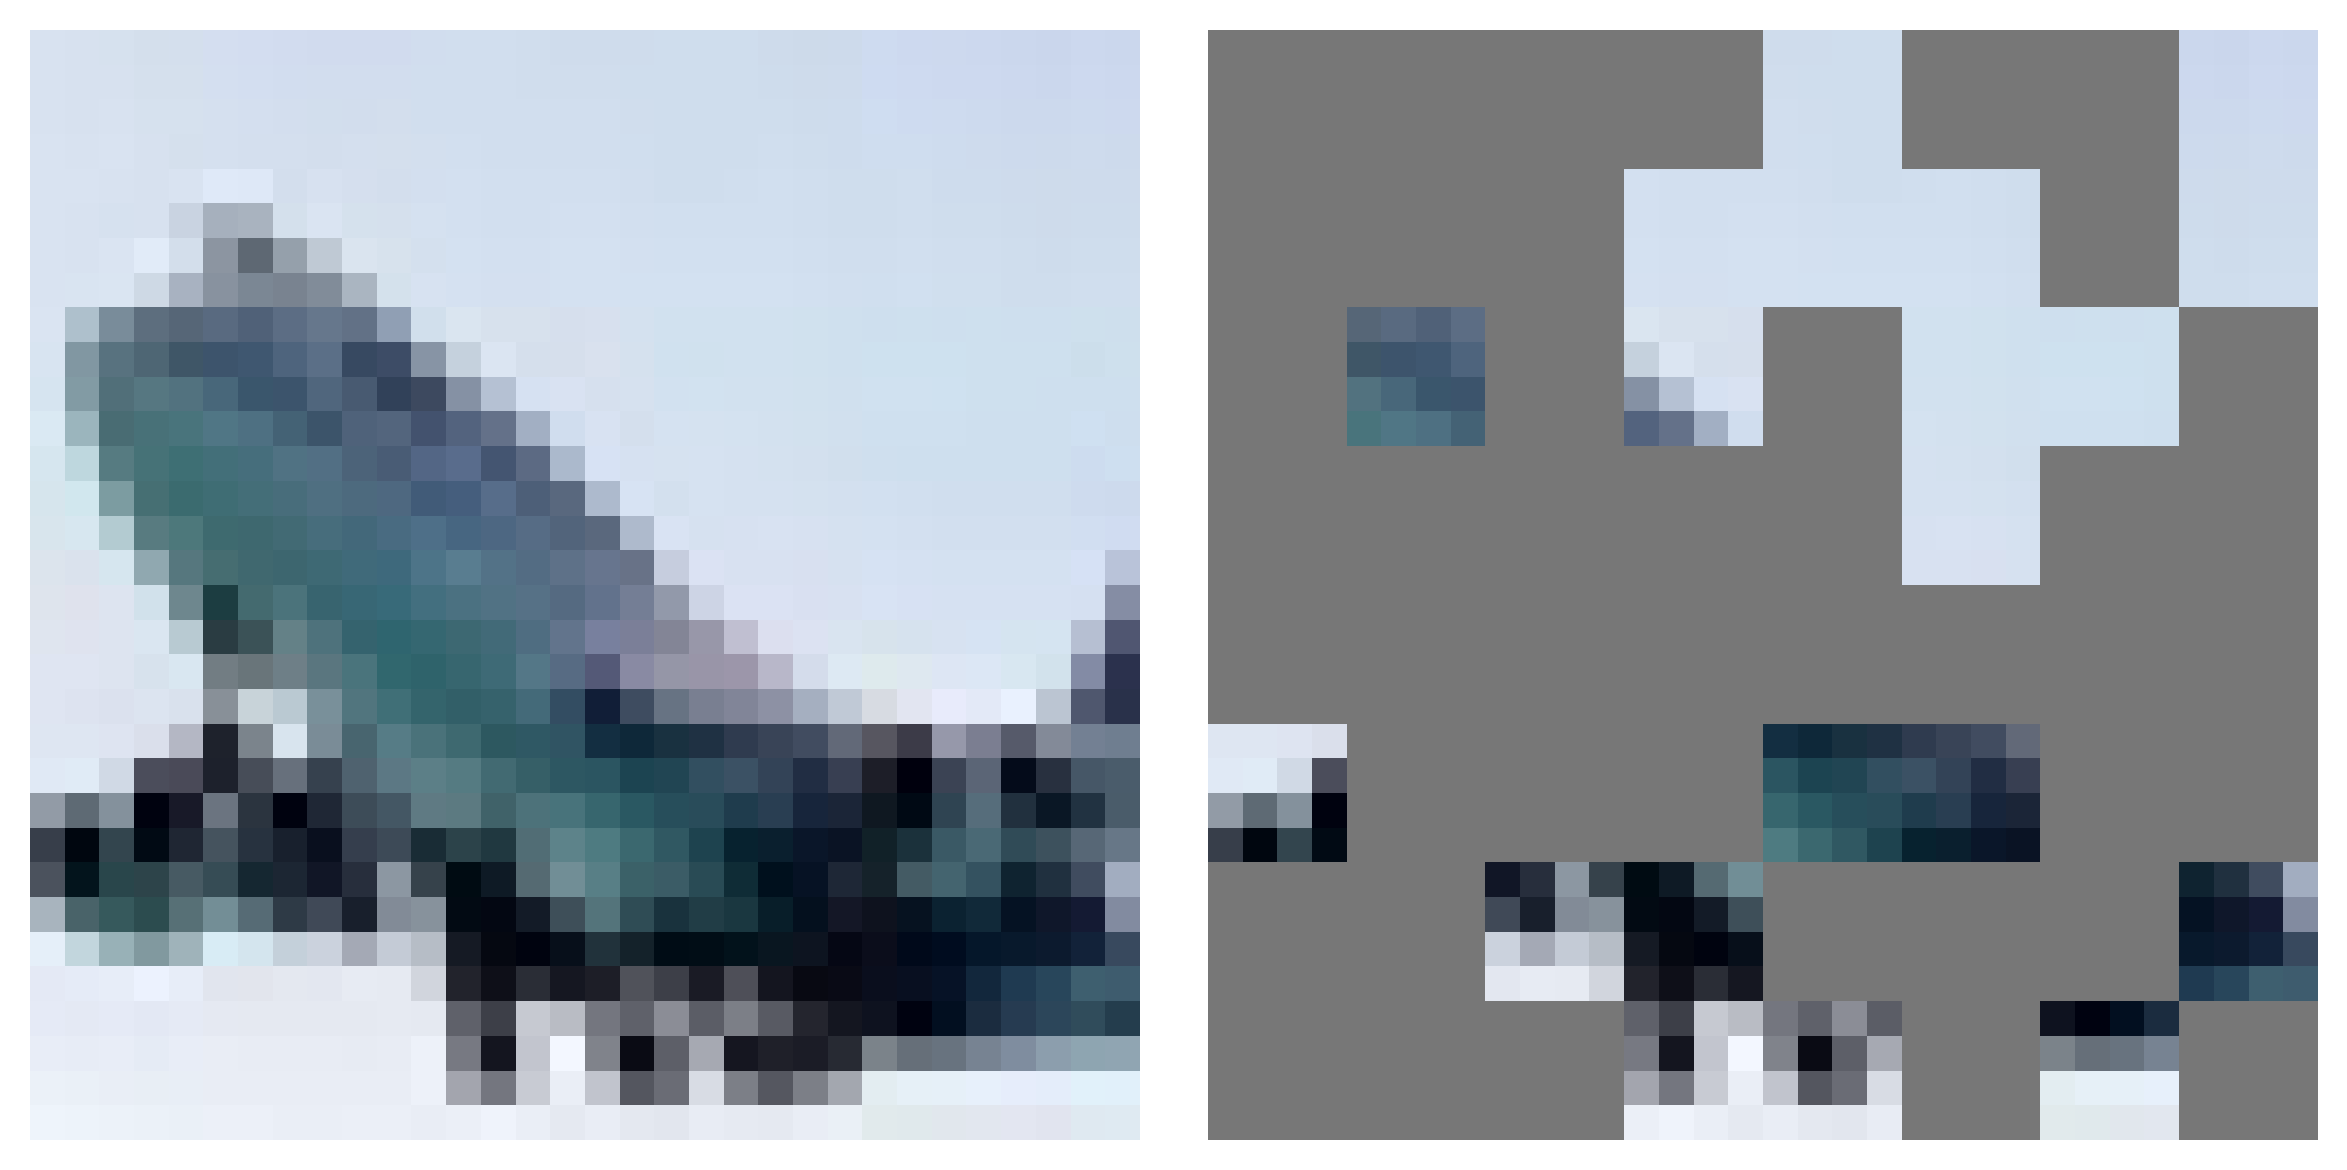
\includegraphics[width=\linewidth]{figures/cifar_mask_example.png}
    \end{minipage}
    \begin{minipage}[t]{0.4\linewidth}
        \centering
        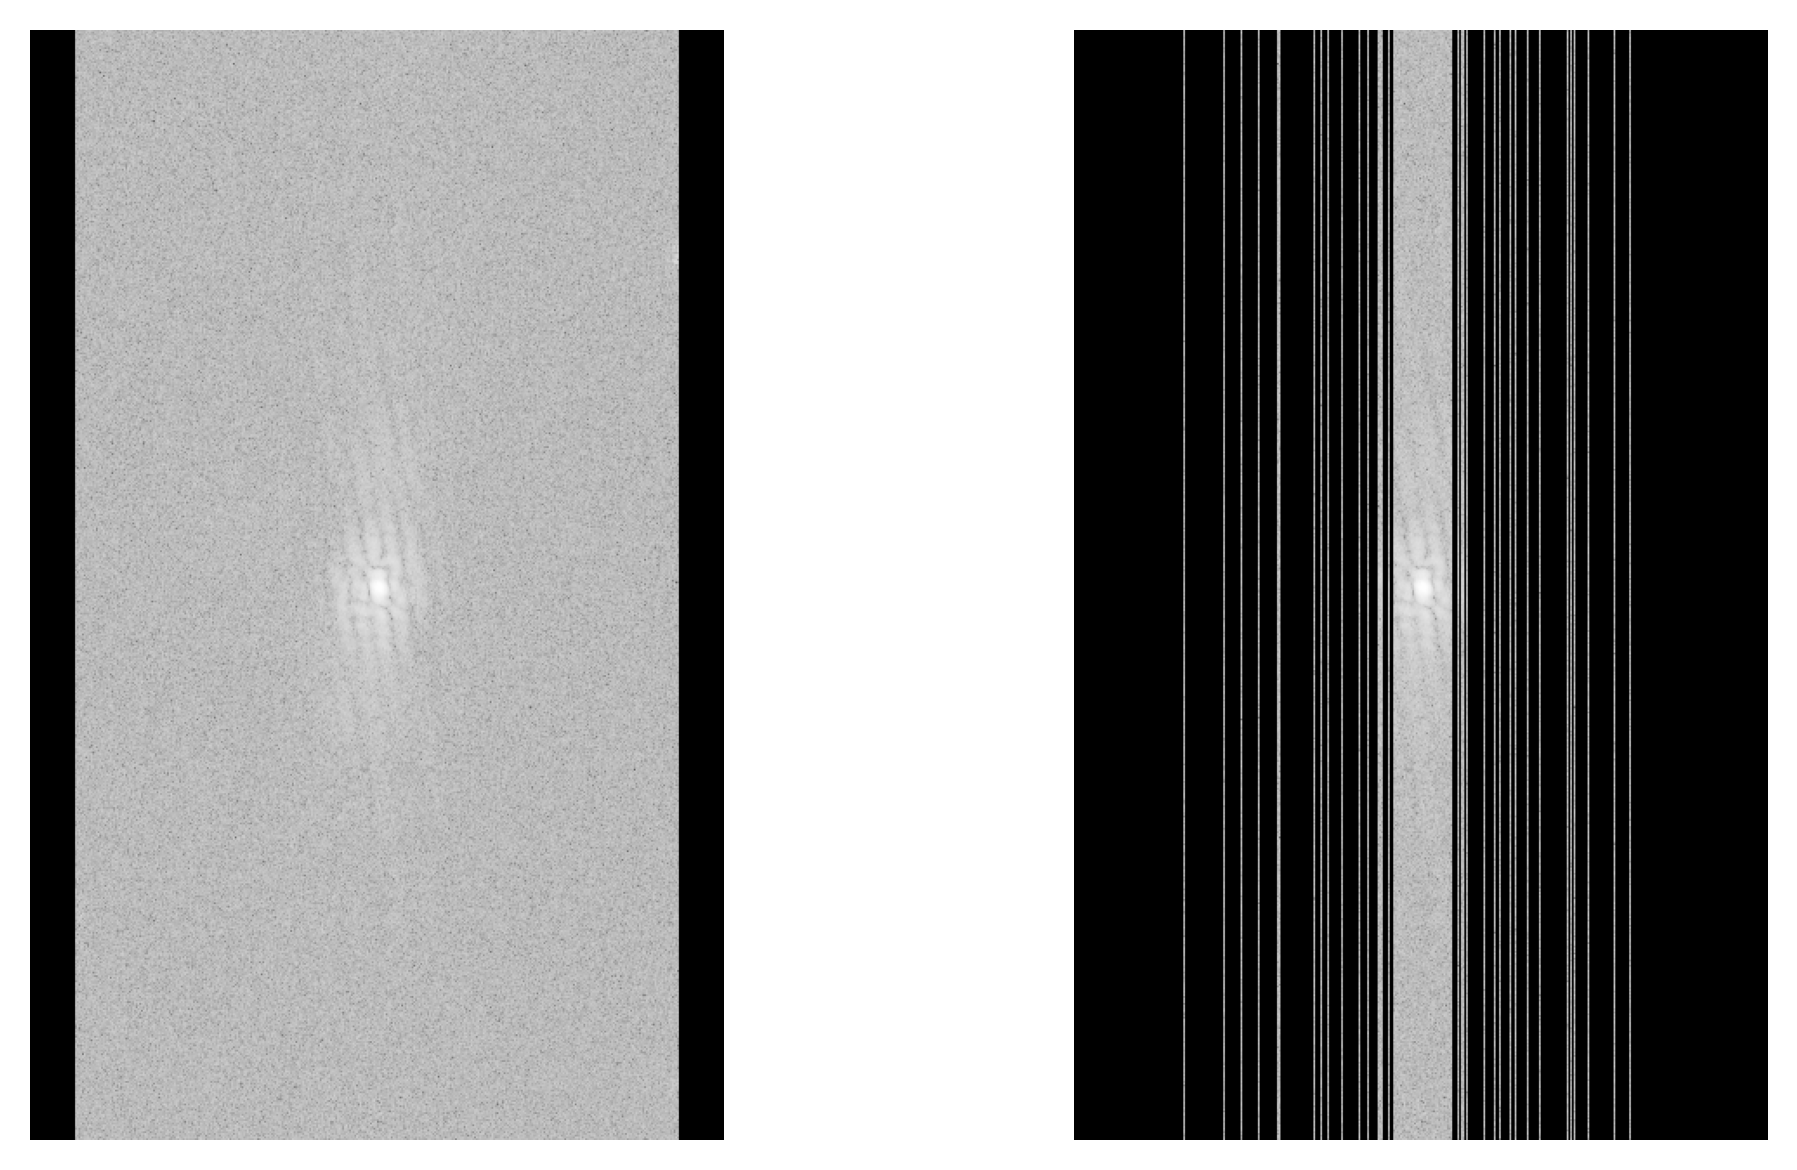
\includegraphics[width=\linewidth]{figures/kspace_mask_example.png}
    \end{minipage}
    \caption{\textbf{Examples of sequential data acquisition in synthetic and \textsc{mr} settings.} 
    \textbf{Left:} in the synthetic regime, the fully observed image $\mbx$ is partitioned into non-overlapping patches, each treated as a feature to be acquired sequentially; the right panel within that image shows the partially observed image $\mbx_t$ after acquisition of $t$ patches. 
    \textbf{Right:} in the \textsc{mr} setting, the left panel shows a fully sampled \textit{k}-space, and the right panel shows the same \textit{k}-space at an intermediate acquisition step.}
    \label{fig:acquisition_examples}
\end{figure}



\subsection{Datasets}
We use the following datasets that span both synthetic and real-world acquisition settings:
\begin{enumerate}[noitemsep]
    \item {\bf CIFAR-10} is a widely used benchmark dataset for image classification, consisting of $60,000$ images of size $32 \times 32 \times 3$ pixels, divided into $10$ object classes, with each class equally represented \citep{cifar10}. 
    
    \item {\bf FastMRI Knee} dataset  \citep{zbontar2018fastmri} provides open-source fully-sampled \textit{k-space} data associated with the knee MR scans. It consists of a total of $41679$ 2D slices, refer to \cref{tab:fastmri_class_stats} in appendices, for the full data statistics. The diagnostic task involves detecting two musculoskeletal abnormalities: {ACL tear} and {meniscus tear}, a standard set of pathologies diagnosed in clinical tasks \citep{singhal2023feasibility,ASMR}. Since these labels are not mutually exclusive, we treat this as a multi-label classification problem.
    
    \item {\bf Clinical Prostate MRI (Internal dataset)} is a large de-identified prostate MRI cohort from an urban health system. The task is binary PI-RADS-positive classification, defined as radiologist-assigned PI-RADS $\geq$ 3, an MRI-based marker of suspicion for clinically significant prostate cancer~\citep{turkbey2019pirads}. Each scan contains an axial T2-weighted volume and diffusion-weighted imaging (DWI). Split statistics and class prevalence are reported in appendices \cref{tab:prostate_dataset_stats}

\end{enumerate}

\subsection{Score Functions}
Our calibration procedures operate on score functions evaluated on a held-out calibration set. We train deep neural network classifiers to obtain these score functions. For CIFAR-10, we train a ResNet-18 \citep{he2016deep} on randomly masked images, to maximize the log likelihood of the associated labels. For the FastMRI Knee and Prostate datasets, we follow the recipe of \citet{singhal2023feasibility} to train classifiers on undersampled $k$-space data.

\begin{figure*}[t]
\centering
    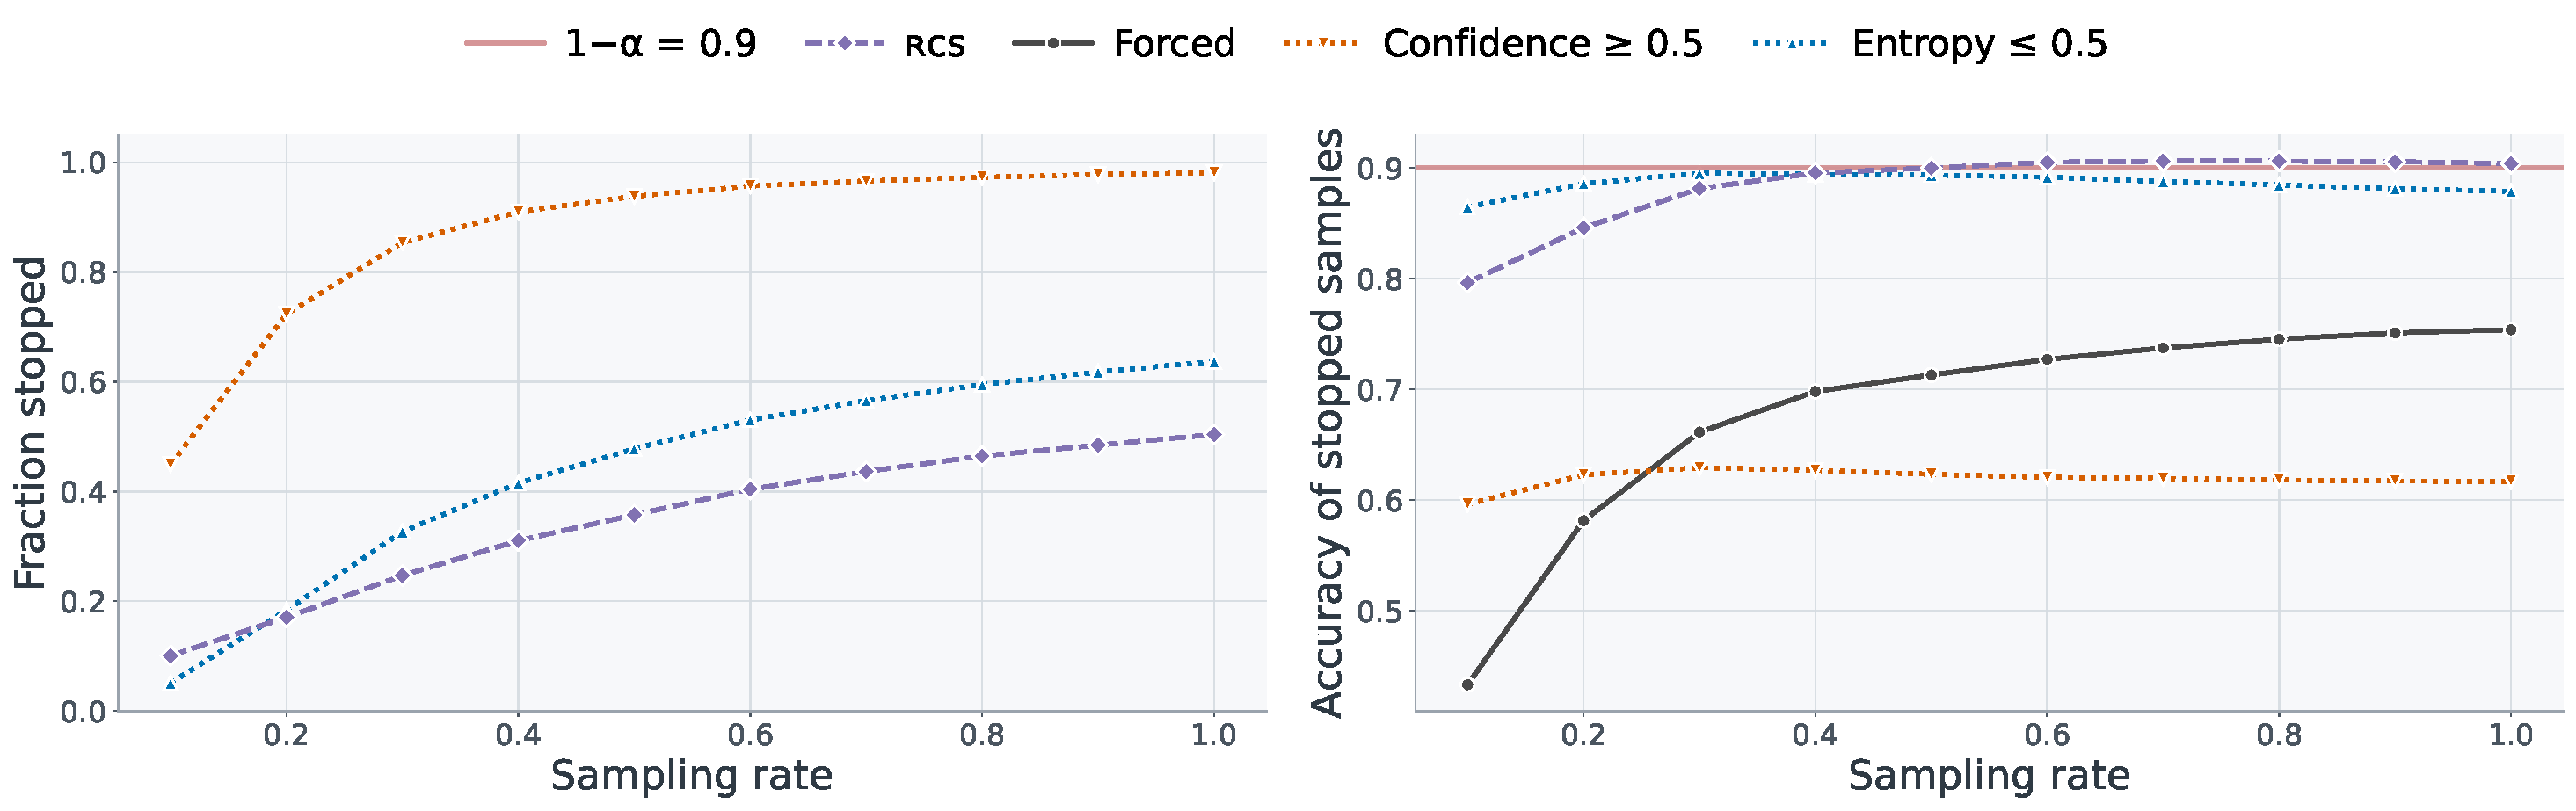
\includegraphics[width=\linewidth]{figures/compare_panel_max_score.pdf}
    \caption{\textbf{Control of misclassification rates on \textsc{CIFAR-10}.} \textbf{Left:} The cumulative fraction of samples halted at each sampling stage. \textbf{Right:} Predictive accuracy of stopped samples as a function of the number of acquired patches. We observe that \gls{method} successfully maintains the misclassification rate below the specified risk level ($\alpha = 0.1$), whereas heuristic baselines consistently violate the safety threshold.}
    \label{fig:cifar-10}
\end{figure*}

\subsection{Evaluation on Sequential Acquisition Tasks}
\label{sec:experiments_1}
We first evaluate the proposed methods on three datasets: CIFAR-10 for object classification with sequential acquisition simulated through patch masking; FastMRI Knee for slice-level musculoskeletal abnormality detection from sequentially acquired $k$-space lines; and Clinical Prostate MRI for PI-RADS-positive classification from sequentially acquired DWI averages, with axial T2 held fixed. 
Examples of the CIFAR-10 and FastMRI Knee acquisition processes appear in \cref{fig:acquisition_examples}. 
For each dataset, we plot the cumulative fraction of examples stopped and the performance on those examples as functions of the acquisition rate. 
We report stopped-sample accuracy for CIFAR-10. 
For FastMRI Knee, we report the class-conditional false negative rate (\textsc{fnr}) among stopped positives for each controlled pathology (ACL tear and meniscus tear) alongside balanced accuracy. 
For Clinical Prostate MRI, we report \textsc{fnr} among stopped PI-RADS-positive exams ($\mathrm{PI\textrm{-}RADS}\geq3$), also alongside balanced accuracy.



% We first evaluate the proposed methods on three datasets, a synthetic task and two clinical tasks.
% \begin{itemize}[noitemsep]
%     \item \textbf{CIFAR-10}: object classification with simulated sequential acquisition via patch masking, see \cref{fig:acquisition_examples}

%     \item \textbf{FastMRI Knee}: slice-level musculoskeletal abnormality detection from sequentially acquired $k$-space lines, see \cref{fig:acquisition_examples}
%     \item \textbf{Clinical Prostate MRI}: PI-RADS-positive classification from sequentially acquired DWI averages, with axial T2 held fixed
% \end{itemize}


\begin{figure*}[h!]
  %\vskip 0.2in
  \begin{center}
    \centerline{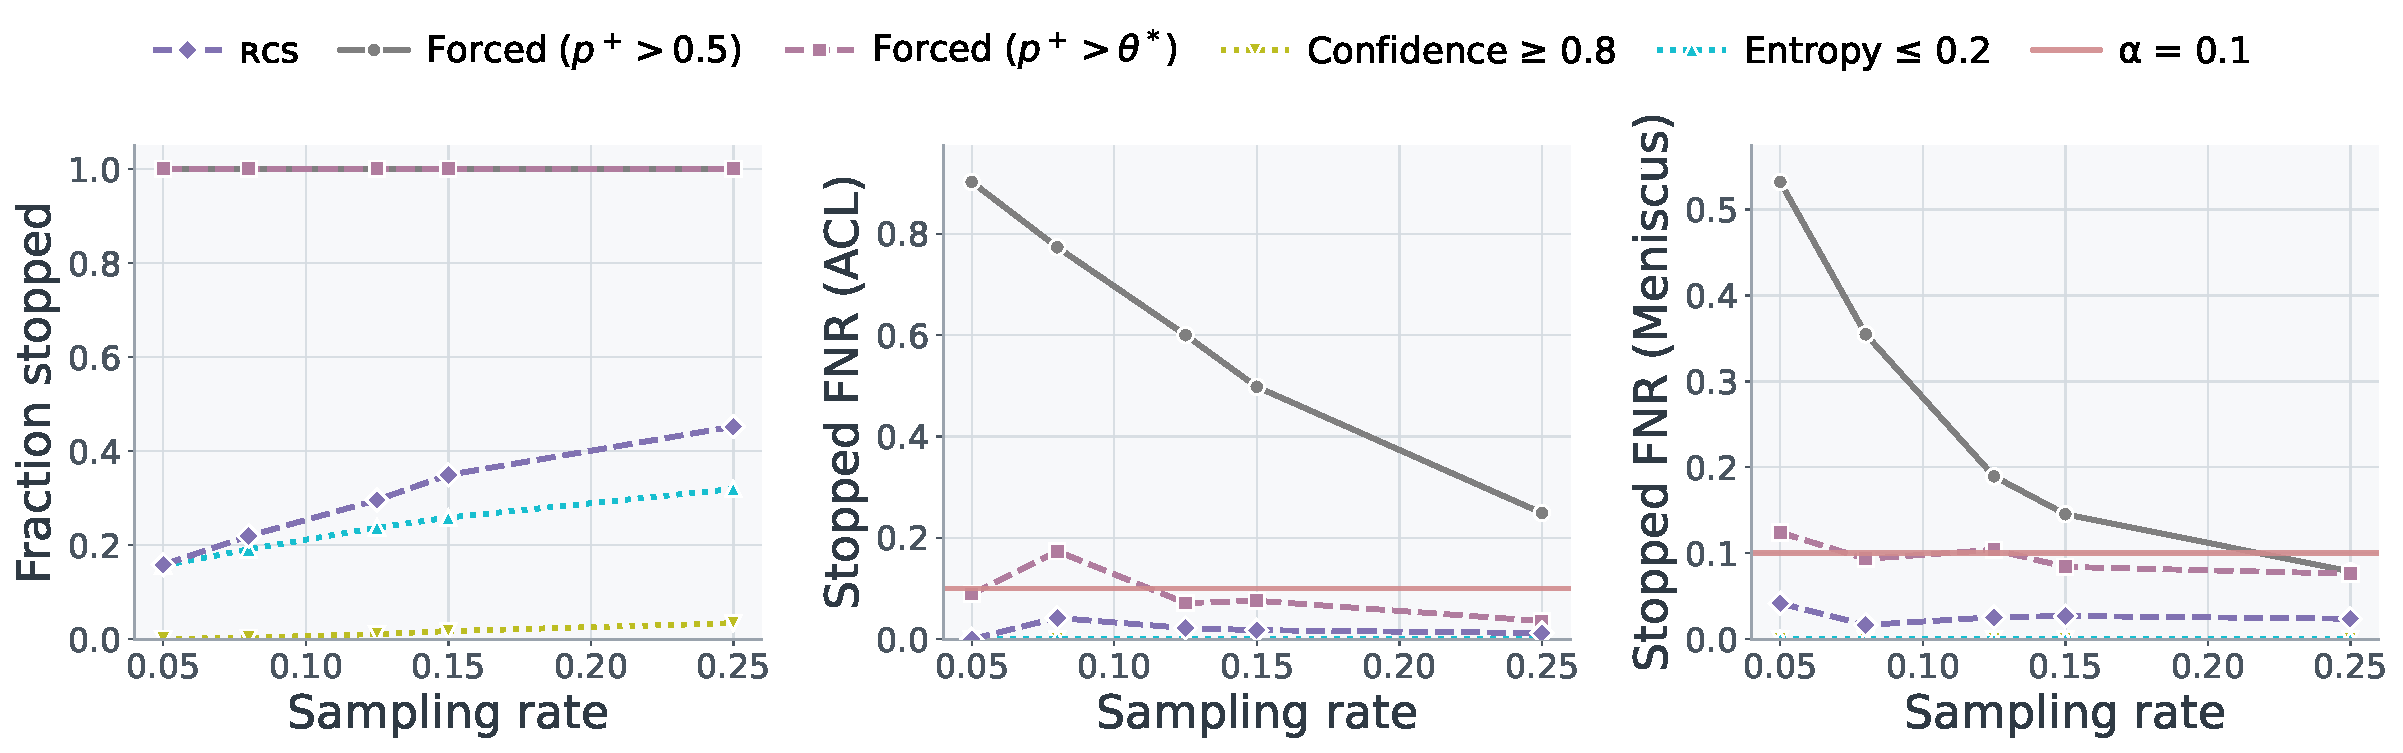
\includegraphics[width=\linewidth]{figures/compare_panel_knee_slice_fnr_conditional_1x3.pdf}}
    \caption{
      \textbf{Class-conditional false negative control on \textsc{FastMRI} knee (\textsc{ACL} tear and meniscus tear).}
      We decide whether to halt slice-level \textit{k}-space collection at sampling rates
      $\cT = \{5\%, 8\%, 12.5\%, 15\%, 25\%\}$.
      The panel reports stopped fraction together with class-conditional \textsc{fnr} among stopped
      positives for \textsc{ACL} tears and meniscus tears
      We observe that \gls{method} controls each pathology-specific \textsc{fnr} at the
      user-specified level ($\alpha = 0.1$) across acquisition rates, including at low
      undersampling such as $5\%$, while heuristic baselines violate the threshold.
      }
      \label{fig:knee-slice-results}
  \end{center}
\end{figure*}


\begin{figure*}[h!]
  %\vskip 0.2in
  \begin{center}
    \centerline{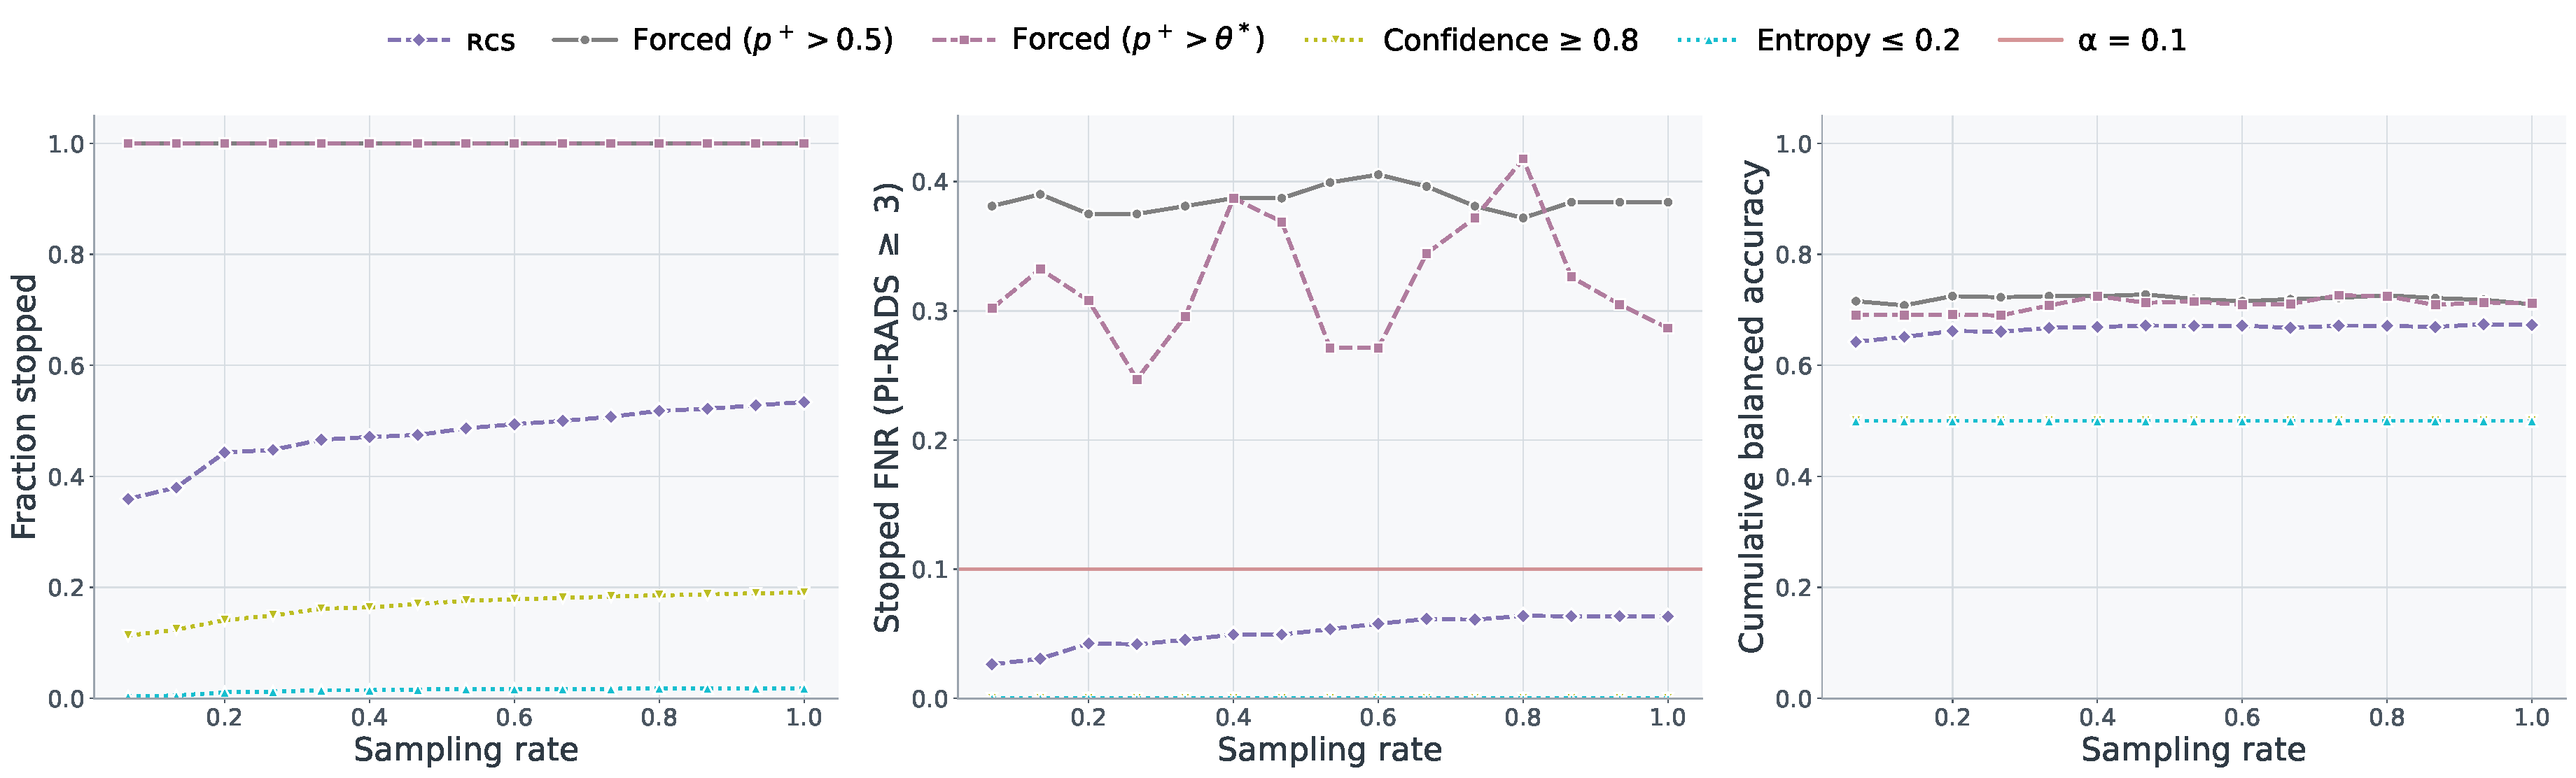
\includegraphics[width=\linewidth]{figures/compare_panel_prostate_pirads_fnr_asym_conditional.pdf}}
    \caption{
      \textbf{Controlling false negative rate (\textsc{fnr}) among stopped exams on Prostate PI-RADS classification.}
      We decide whether to halt acquiring diffusion averages for DWI sequences along the scanner-ordered
      reconstruction checkpoints.
      \textbf{Left:} fraction of exams stopped by \gls{method} and heuristic criteria.
      \textbf{Center/Right:} \textsc{fnr} and balanced accuracy on the stopped cohort, where the controlled
      risk is the false-negative rate among PI-RADS-positive exams ($\mathrm{PI\textrm{-}RADS}\!\geq\!3$)
      that have already been halted.
      We observe that \gls{method} maintains this stopped-sample \textsc{fnr} at the user-specified level
      ($\alpha = 0.1$) across acquisition stages, whereas baseline strategies violate the safety threshold.}
      \label{fig:prostate-results}
  \end{center}
\end{figure*}

% \paragraph{Evaluations.} For each dataset, we plot:
% \begin{enumerate}
%     \item \textbf{Stopped fraction v/s acquisition rate:} the cumulative fraction of examples for which acquisition has been halted by each acquisition time
%     \item \textbf{Stopped-sample performance v/s acquisition rate:} the performance of the subset of stopped examples, measured by the task-relevant risk criteria.
% \end{enumerate}
% For CIFAR-10, we report stopped-sample accuracy. For FastMRI knee, we report \emph{class-conditional} false negative rate (\textsc{fnr}) among stopped positives for each controlled pathology (ACL tear and meniscus tear), together with balanced accuracy. For Clinical Prostate MRI, we report \textsc{fnr} among stopped PI-RADS-positive exams ($\mathrm{PI\textrm{-}RADS}\!\geq\!3$), again alongside balanced accuracy.

\paragraph{Acquisition setup.} For CIFAR-10, we simulate sequential acquisition by partitioning each image into $4 \times 4$ non-overlapping patches and acquiring these patches progressively over time. For the knee MRI dataset, we simulate sequential acquisition directly in the raw $k$-space domain, where each acquisition step reveals additional frequency-domain lines. This matches the underlying measurement process and allows us to evaluate stopping decisions in a clinically realistic acquisition regime.
For Clinical Prostate MRI, sequential acquisition follows the scanner order of the DWI sequence. The axial T2-weighted volume is acquired before the DWI sequence and is fixed across all states. The full DWI protocol contains 48 acquired DWI measurements: 12 at $b=50\,\mathrm{s/mm^2}$, with 4 repeats per diffusion direction, and 36 at $b=1000\,\mathrm{s/mm^2}$, with 12 repeats per direction. Stopping policies are evaluated at 15 scanner-ordered reconstruction checkpoints. At each checkpoint, ADC and computed high-$b$ ($b=1500\,\mathrm{s/mm^2}$) DWI volumes are reconstructed only from the measurements acquired so far, consistent with PI-RADS v2.1 guidance~\citep{turkbey2019pirads}. Later checkpoints therefore contain progressively higher-SNR diffusion information. A fixed 3D T2+DWI fusion classifier produces a PI-RADS-positive score at each checkpoint~\citep{johnson2025prostate}. Appendix Figure~\ref{fig:prostate_dwi_acquisition_states} visualizes DWI-derived reconstructions across the acquisition trajectory.

\paragraph{Baselines.} As baselines, we compare \gls{method} to three potentially ``unsafe" strategies. 
First, \textbf{Forced with Static Decision Thresholds} where the model is forced to make a prediction for every sample across all sampling rates. 
The score threshold used to generate the prediction is a static scalar (we use $p^+ > 0.5$).
This is referred to as ``Forced ($p^+ > 0.5$)" in  Figures \ref{fig:knee-slice-results} and \ref{fig:prostate-results}.
Second, \textbf{Forced with Calibrated Decision Thresholds} where the model is forced to make a prediction for every sample across all sampling rates. 
The score threshold used to make a prediction at each sampling rate is calibrated to maximize some metric of interest (we use balanced accuracy). 
This is referred to as ``Forced ($p^+ > \theta^*$)" in Figures \ref{fig:knee-slice-results} and \ref{fig:prostate-results}.
Third, \textbf{Heuristic Stopping Thresholds} determine dynamic stopping times based on some heuristic threshold on the scores. 
We use Confidence and Entropy of the predictions.


\paragraph{Results.} 
For our synthetic CIFAR-10 experiment, we use the misclassification rate as the risk ($R(y, C_{\alpha}(\mbx_t, t)) = \mathbf{I}(y \not\in C_\alpha(\mbx_t, t))$), and control it at the rate of $10\%$ ($\alpha=0.1$), implying a target coverage/accuracy of $90\%$. 
For both datasets, we report performance as a function of the percentage of features acquired (a.k.a., the acquisition rate) and at every acquisition rate, we track the cumulative percentage of stopped samples. 
This is a direct indicator of our proposed guarantee: for all stopped samples, we maintain an accuracy level corresponding to the input miss-coverage rate ($\alpha$). We compare the performance of \gls{method} against the Fixed Sampling Rate Stopping or ``Forced", Confidence-based Thresholding, and Entropy-based Thresholding. See Figure~\ref{fig:cifar-10} for results on \textsc{cifar-10} dataset. Thresholds for the Entropy and Confidence baselines are set to $0.5$.

In our clinical diagnosis tasks, the risk of interest is false-negative error among sample that have been stopped.
For FastMRI knee, this is instantiated as a \emph{class-conditional} multi-label guarantee: we control pathology-specific \textsc{fnr} for ACL tear and meniscus tear separately, and we report the corresponding per-pathology curves in \cref{fig:knee-slice-results}.
For Prostate PI-RADS, the task is binary, so the same stopped-sample \textsc{fnr} reduces to control among PI-RADS-positive exams in \cref{fig:prostate-results}.

We instantiate $\cD_\textsc{stop}(\mbx_t; \lambda)$ using \emph{ambiguity-band stopping rules}. For each acquisition time $t$ and task $k$, we define an uncertainty interval $[\ell_{t,k}(\lambda), u_{t,k}(\lambda)]$. The parameter $\lambda \in [0, 1]$ scales the band's width, interpolating from maximal ambiguity (highly conservative) to a narrow, data-driven baseline (aggressive). The policy halts acquisition at the first step where predictive scores for \emph{all} controlled tasks exit their respective bands, assigning terminal predictions based on the side of the exit. While we detail this specific band construction in Appendix \ref{app:ambiguity_bands}, our \gls{method} guarantees remain valid for any arbitrary stopping rule parameterized by $\lambda$. 

In \cref{fig:knee-slice-results,fig:prostate-results} we observe that \gls{method} shows efficient stopping behavior while always adhering to the risk constraint. Furthermore, across both sets of experiments, we observe that even though the baseline method ``Forced ($p^+ > \theta^*$)" is calibrated to maximize the balanced accuracy, \gls{method} shows comparable performance while never violating the risk threshold.

\paragraph{Sensitivity to the risk level $\alpha$.}
Beyond fixed operating points, we study how stopping behavior changes as the user varies the allowed risk $\alpha$.
For each $\alpha$ on a grid, we re-select the certified threshold $\widehat{\lambda}(\alpha)$ on the same calibration scores and evaluate the resulting policy on the held-out test set.
\cref{fig:alpha-sweep} summarizes these sweeps for FastMRI knee and Prostate PI-RADS.
The top panels show the cumulative stopped fraction versus acquisition rate, with one curve per $\alpha$: larger $\alpha$ (more permissive risk) yields earlier and more frequent stopping.
The bottom panel reports the expected acquisition rate at stopping, $\mathbb{E}[r_{\mathrm{stop}}]$, as a function of $\alpha$, quantifying the efficiency--risk tradeoff induced by calibration.
As expected, $\mathbb{E}[r_{\mathrm{stop}}]$ decreases monotonically as $\alpha$ increases, while the fixed-$\alpha$ panels above confirm that the corresponding stopped cohorts remain consistent with the requested risk level.

\begin{figure*}[t]
  \vskip 0.2in
  \begin{center}
    \centerline{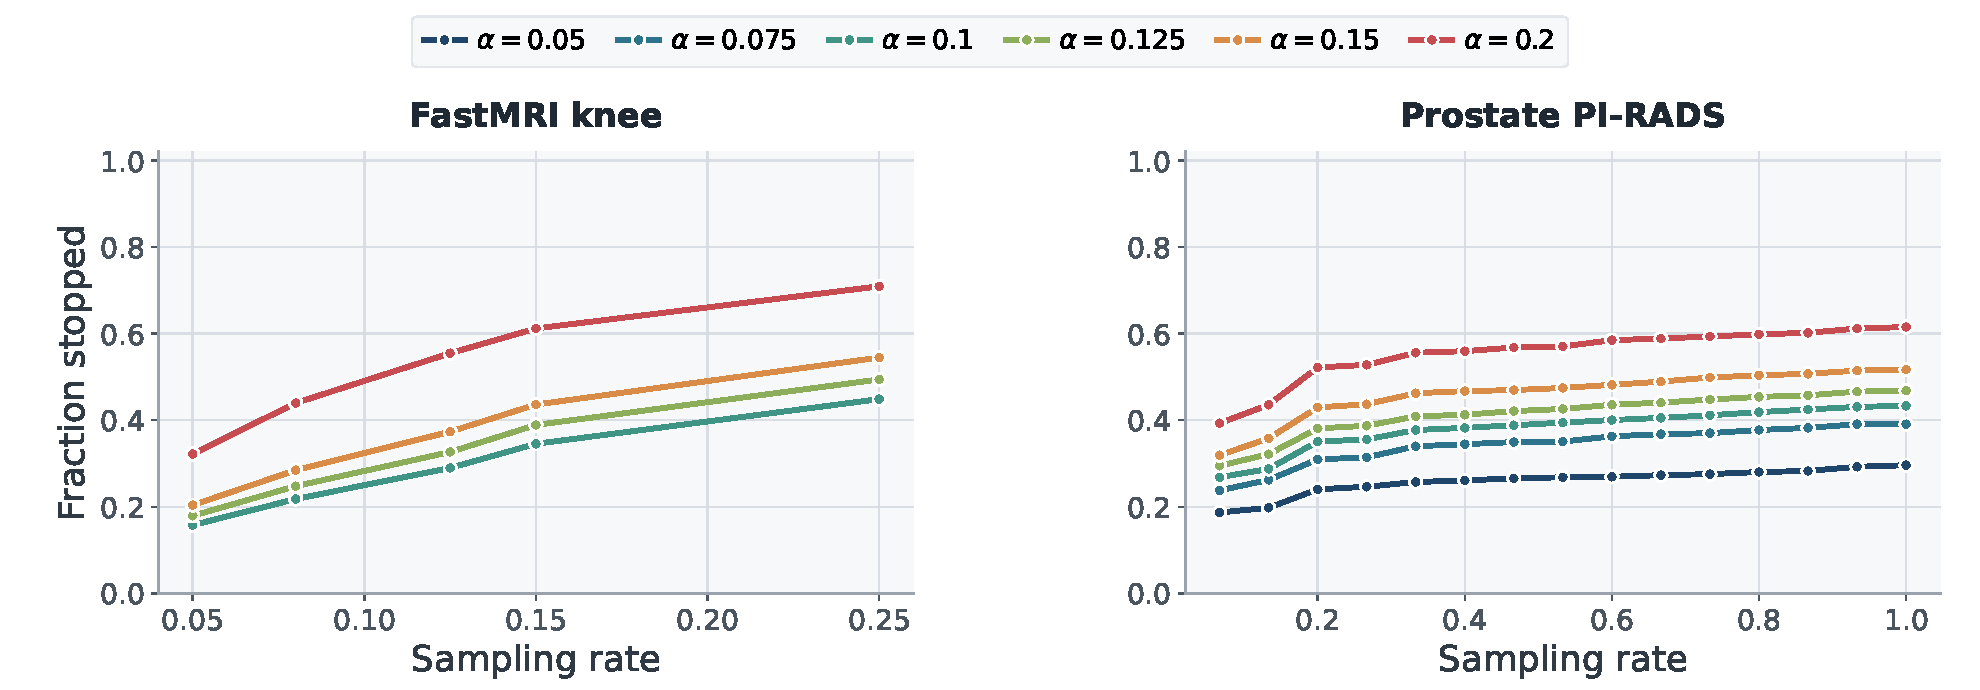
\includegraphics[width=\linewidth]{figures/alpha_stopping_mri_panel_top.pdf}}

    \vspace{0.1in}
    \centerline{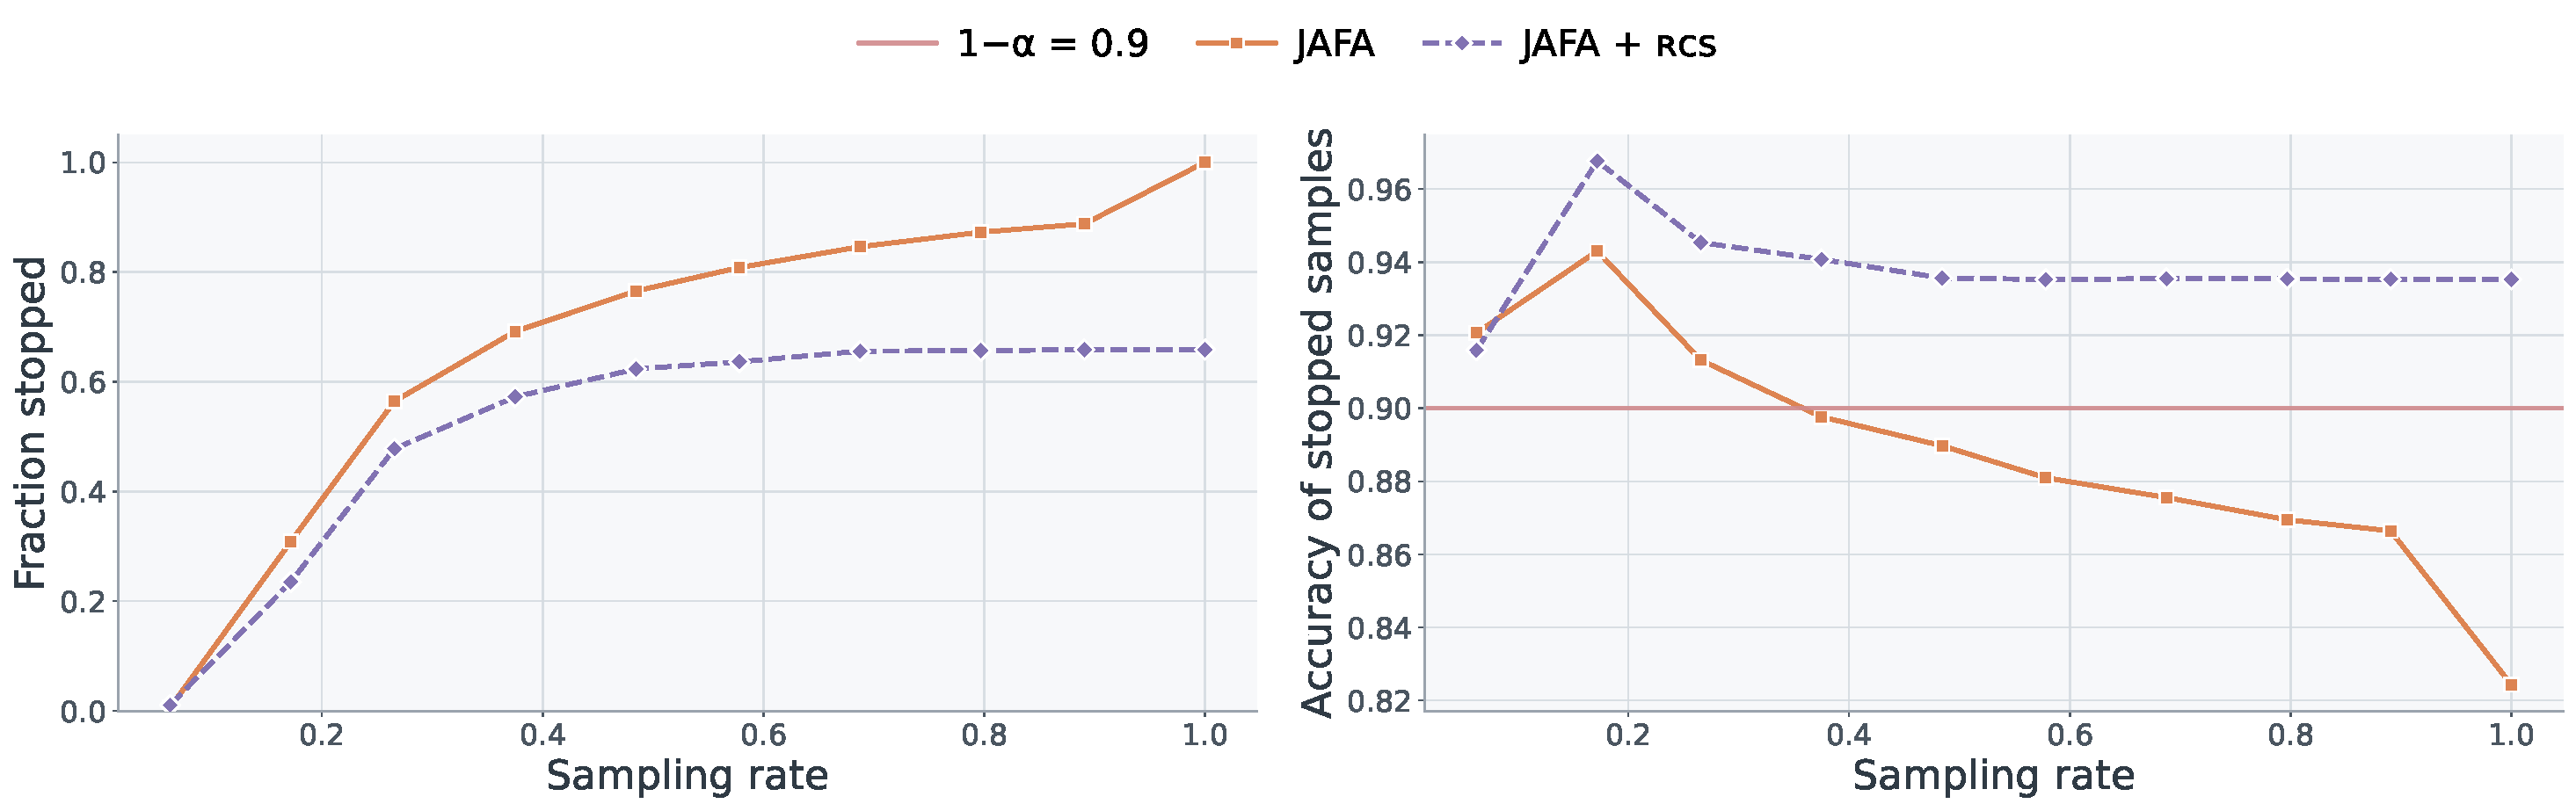
\includegraphics[width=0.9\linewidth]{figures/compare_panel_max_score_q_margin_max.pdf}}
    
    \caption{
      {\bf Upper Panel:} \textbf{Effect of the risk level $\alpha$ on calibrated stopping (FastMRI knee and Prostate PI-RADS).}
      We show the cumulative fraction of stopped examples versus sampling rate for several values of $\alpha$
      (one curve per $\alpha$).
      {\bf Lower Panel:}
  \textbf{Complementing a learned acquisition policy with \gls{method} (CIFAR-10).} In this experiment we wrap JAFA \citep{jafa-2018} with \gls{method}, and compare the efficiency and safety of the resulting policy with JAFA alone. In the left plot, we plot the fraction of samples stopped by each procedure across acquisition stages. In the right plot, we monitor the risk (miscoverage) of both across acquisition stages. We observe that at the cost of slightly lower efficiency, JAFA+\gls{method} adheres to the safety constraint while JAFA alone does not.
      }
      \label{fig:alpha-sweep}
  \end{center}
\end{figure*}


\subsection{Compatibility with Adaptive Acquisition Policies}
\label{sec:experiments_2}
Our second set of experiments evaluate whether the proposed stopping-calibration procedures can serve as post hoc wrappers on top of learned adaptive acquisition policies. Since our method is designed to be agnostic to the acquisition mechanism itself, it should be applicable not only to fixed or random acquisition trajectories, but also to learned adaptive policies, provided that the calibration and test trajectories are sampled from the same induced distribution.
To demonstrate this, we use \textbf{JAFA} \citep{jafa-2018}, a reinforcement-learning-based adaptive feature acquisition method that jointly learns which feature to acquire next and when to stop. JAFA provides a strong representative of the adaptive acquisition literature, in which acquisition decisions are optimized for average utility or reward but are not, by themselves, equipped with post hoc statistical guarantees on the risk of the final stopped decision.

\paragraph{Wrapper construction}
We treat JAFA as an acquisition backbone and construct a parameterized stopping wrapper on top of it. Concretely, JAFA generates a sequential acquisition trajectory and exposes a stopping score at each acquisition step. Specifically, JAFA learns a Deep-Q network, that produces values for a given $(\text{state},\text{action})$ pair. The policy selects the next action by picking $a_{t+1} = \argmax_a Q(a,s_t)$, where $Q$ is the Q-network and $s$ is the state at time $t$. By taking the difference between the Q-value for the "STOP" action and the argmax action (excluding $a_{t+1} = \text{"STOP"}$), we can define a score function. We then instantiate a family of wrapped stopping policies by thresholding this score with a tunable parameter $\lambda$, and apply \gls{method} to select a risk-certified member of this wrapped family. This preserves JAFA's adaptive acquisition behavior while calibrating the final decision to satisfy a user-specified risk target.

% \begin{figure*}[h!]
%   \vskip 0.2in
%   \begin{center}
%     \centerline{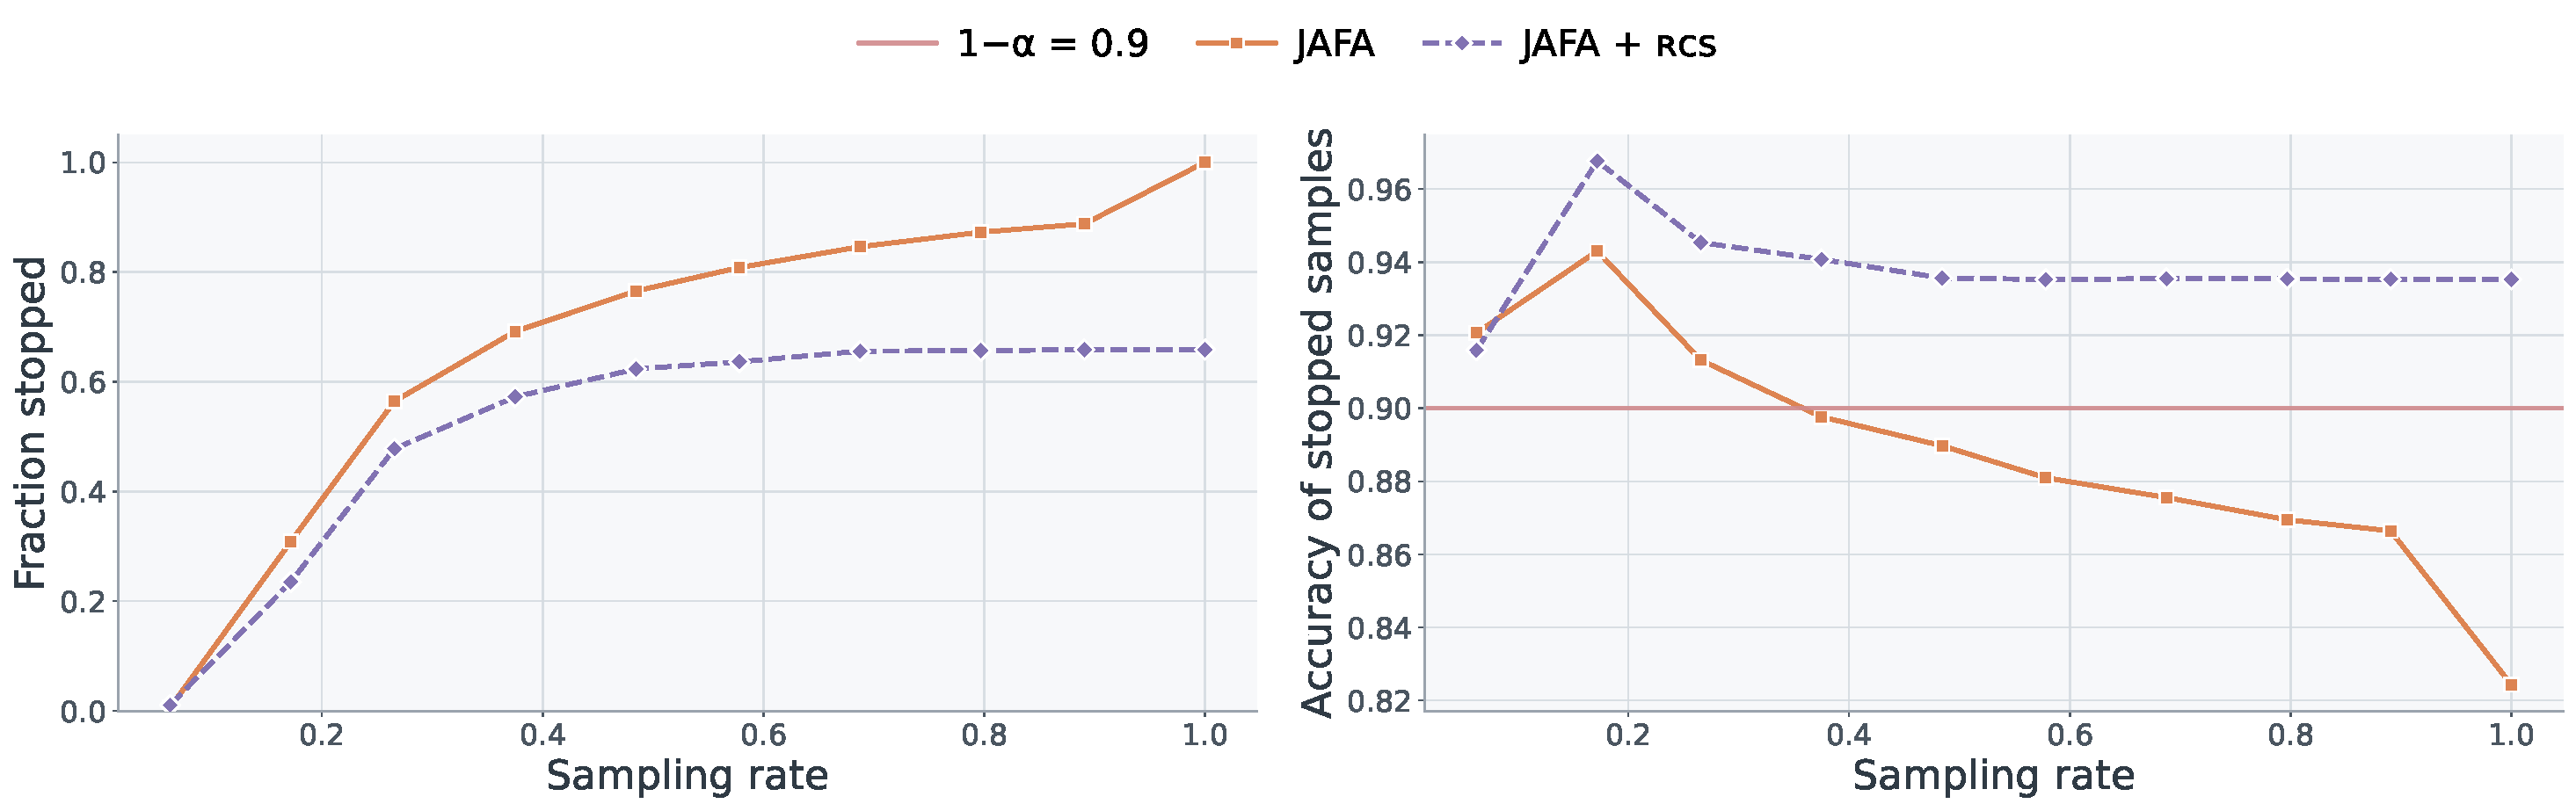
\includegraphics[width=\linewidth]{figures/compare_panel_max_score_q_margin_max.pdf}}
%     \caption{
%       \textbf{Complementing a learned acquisition policy with \gls{method}.} In this experiment we wrap JAFA \citep{jafa-2018} with \gls{method}, and compare the efficiency and safety of the resulting policy with JAFA alone. In the left plot, we plot the fraction of samples stopped by each procedure across acquisition stages. In the right plot, we monitor the risk (miscoverage) of both across acquisition stages. We observe that at the cost of slightly lower efficiency, JAFA+\gls{method} adheres to the safety constraint while JAFA alone does not.
%       }
%     \label{fig:cifar-jafa}
%   \end{center}
% \end{figure*}

\paragraph{Results.}
To isolate the effect of the wrapper cleanly, we perform this experiment on \textbf{CIFAR-10} only. As in \ref{sec:experiments_1}, we report: 1)  the cumulative fraction of stopped samples versus acquisition rate, and 2) he stopped-sample performance versus acquisition rate.
From \cref{fig:alpha-sweep} (lower panel), 
%\cref{fig:cifar-jafa}, 
we observe that calibrating on JAFA-generated acquisition trajectories enhances the efficiency of the stopping procedure. At the same time, our wrapper ensures that the accuracy of the stopped samples remains above $90\%$. Because both methods use the same underlying predictor, \gls{method} achieves this result by abstaining on the few samples that JAFA would otherwise misclassify.

\section{Discussion}
In this work, we introduce risk-controlled stopping (\textsc{rcs}), a method to safely stop data acquisition in sequential classification tasks. \gls{method} provides post-hoc, distribution-free risk control at user desired thresholds and notions of risk. These risk functions and thresholds can be changed without requiring any further training. Our experiments on the \textsc{fastMRI} knee and the prostate dataset show that \gls{method} can significantly accelerate clinical decision making pipelines, while rigorously controlling class-conditional (or stopped-sample) false-negative risk despite accelerations. Furthermore, we demonstrate that \gls{method} is complementary to learned acquisition policies, and provides rigorous statistical guarantees on their behavior. 

\subsection{Limitations}
Producing the \gls{method} guarantee requires access to fully-sampled data or data sampled from the same policy. However, in future work, we plan on using masked data that could be collected during a deployment of early stopping methods. Moreover, the class of policies parameterized by $\lambda$ could be enriched by allowing $\lambda$ to be multi-dimensional, thereby capturing the strong correlation structure among errors across nearby acquisition steps.